\documentclass[preprint,12pt,times]{elsarticle}
\usepackage[utf8]{inputenc} \usepackage{amsmath}
\usepackage[margin=1in]{geometry} \usepackage{graphicx} \usepackage{epstopdf} \usepackage{setspace} \usepackage{amsthm} \usepackage{comment} \usepackage{pgfplots}\usepackage{longtable}
\usepackage{indentfirst}\doublespacing \usepackage{soul}

\begin{document}

\begin{center}
\vspace*{5cm}

        \begin{Large}
        {M.S. Technical Paper}
        \end{Large}
        
        \vspace{1cm}
        \begin{LARGE}
        \textbf{An Initial Analysis of Demand and The Difference in Ticket Prices for Clemson Basketball Games}
        \end{LARGE}
        
        \vspace{10cm}
        \begin{Large}
        Tim Mango
        \end{Large}
        
        \begin{Large}
        M.S. Applied Economics and Statistics
        \end{Large}
        
        \begin{Large}
        Clemson University
        \end{Large}
        \vspace{0.1cm}
        
        \begin{Large}
        Spring 2019
        \end{Large}
        \vfill
\end{center}

\newpage

\begin{large}
\noindent\textbf{A letter to my committee:}
\end{large}

I have had the privilege of earning my B.S. in Economics from Clemson University and I am excited to finish my M.S. in Applied Economics and Statistics from the same institution.  This paper is designed to demonstrate skills I have learned through coursework and work experience in economics, statistics, and data science.

Margeret Rose defines data science as: “The study of where information comes from, what it represents and how it can be turned into a valuable resource in the creation of business and IT strategies. Mining large amounts of structured and unstructured data to identify patterns can help an organization rein in costs, increase efficiencies, recognize new market opportunities and increase the organization's competitive advantage.”

The motivation for this technical paper was found while I was working on a project for Clemson Athletics and Clemson Men's Basketball.  The initial goal was to explore Clemson Athletics data and look for opportunities to increase revenues and maintain or strengthen customer relationships.  After some investigation, I discovered that third party ticket vendors were pricing Men's Basketball tickets significantly higher than the Athletic Department, particularly for high demand games.  I became interested in third party ticket pricing and thought it might be interesting to model ticket pricing for Clemson Men's Basketball games from an economic approach.

I remembered reading several papers in one of my graduate courses, Sports Economics, that provided estimates of elasticity of demand for sports events.  I also knew that estimates of elasticity of demand can provide insight for maximizing revenue with prices.  For proprietary reasons, I cannot use Clemson data in this paper. However, I model hypothetical demand and elasticity of demand estimates for Clemson Men's Basketball games as a proposed explanation for the difference in ticket prices.  The models are conceptual and more data is needed to discover the source of the difference in ticket prices.  I also gathered a large dataset of division 1 basketball attendance records and the dataset is used to investigate variables that influence attendance for Clemson Men's Basketball games.

\newpage
\begin{large}
\noindent\textbf{Business Case}
\end{large}

Universities have both a symbiotic and parasitic relationship with third party ticket vendors. Third party ticket vendors add value by creating a convenient marketplace of exchange for tickets.  However, third party vendors charge fees and higher prices for products that are provided by universities and their athletic programs. Universities rarely capture the added revenue generated by ticket vendors in the secondary market.

One explanation for the difference in ticket prices is the difference in organizational structures of universities and third party ticket vendors.  Ticket vendors are profit maximizing businesses while universities are designed to enrich student experience, maintain alumni connections, and support education.  Another explanation is that third party ticket vendors have a better understanding of the demand for university sports events, and universities are missing out on ticket revenue.  Within the context of Clemson Men's Basketball, two questions arise from the business case.  What is the demand for a Clemson Men's Basketball game?  Given the demand for the game, what ticket prices maximize revenue?  Hypothetical estimates of demand and elasticity of demand for low demand basketball games, average demand basketball games, and high demand basketball games are presented to provide an exploratory framework for the business case questions.\\

\begin{large}
\noindent\textbf{Surveying Economic Literature}
\end{large}

\noindent\textbf{Estimating Demand}

Noll (1974) and Demmart (1973) wrote some of the first papers studying the factors that determine stadium attendance.  The primary variables investigated in these papers were income levels in the local marketplace, population in local stadium areas, quality of the sports teams playing in the stadium, ticket price, and availability of substitutes (alternative entertainment options) for stadium attendance.  Patrick Feehan (2006) expands on these models and he claims that stadium attendance can also be affected by factors such as habit of persistence (return customers) and the degree of outcome uncertainty of the sports event.

Feehan defines three types of outcome uncertainty.  The first type of uncertainty is long-run uncertainty.  This is where a small group of teams dominate a league over a sustained period of time.  The effect of this type of uncertainty is diminished attendance for low performing teams and eventually lower attendance for successful teams, which he claims is a result of a satiation effect.  The second type of uncertainty relates to the outcome of an individual game.  This suggests higher attendance at games having higher amounts of uncertainty and lower attendance at games having lower amounts of uncertainty. The final type of uncertainty relates to the identity of a conference or season champion.  Attendance is expected to be higher if the outcome of a game can determine a conference or season champion.  This is further discussed by Jennett (1984) in his paper on the uncertainty of outcomes in Scottish soccer leagues.\\

\noindent
\textbf{Elasticity of Demand}

Elasticity of Demand shows how sensitive consumers are to changes in price.  For normal goods, an increase in price leads to a decrease in quantity demanded, and this is the scenario explored in this paper.  Rascher, Mcevoy, Nagel, and Brown (2007) wrote a paper on variable pricing for Major League Baseball.  This would enable teams to change ticket prices during the season, which is an area that is already leveraged by third party ticket vendors.  Several of the factors that affect pricing are quality of the opponent, day of the week, month of the year, and special events (opening day, holidays, etc.).  Cameron (2002) sites the Colorado Rockies having four different prices for the same seat throughout the course of the season.

Elasticity of demand can be used as a tool to help determine ticket prices for different game conditions and event dates throughout the season.  Noll (1974) had point estimates of elasticity for baseball games in the inelastic range (-0.49) and Scully (1989) also had inelastic point estimates (-0.63 and -0.76).  Boyd and Boyd (1996), however, measured point estimates ranging from inelastic (-0.58) to elastic (-1.20) after controlling for increases in attendance due to the effects of a home field advantage.  As an example, an elasticity of -0.49 is interpreted as a 0.49 percent decrease in quantity demanded relative to a 1 percent increase in price.  An elasticity of -1.2 is interpreted as a 1.2 percent decrease in quantity demanded relative to a 1 percent increase in price. Many studies have found baseball game demand to be inelastic, but some games may have an elastic demand.  The next section discusses how knowledge of demand and elasticity of demand can be used to maximize sport ticket revenue.\\

\begin{Large}
\noindent\textbf{\ul{Maximizing Revenue With Demand and Elasticity of Demand}}
\end{Large}
\begin{large}
\begin{enumerate}
  \item Elasticity of Demand Overview
  \item Measuring Elasticity of Demand with a Demand Shift or Demand Slope Change
  \item Measuring Elasticity of Demand Along a Demand Curve
  \item Maximizing Revenue with Elasticity of Demand
  \item Proposed Model of Clemson and Third Party Ticket Pricing
\end{enumerate}
\end{large}

\section {\textbf{Elasticity of Demand Overview}}

Elasticity of demand is defined as the percentage change in quantity demanded for a product relative to a one percent change in the price for a product. Elasticity of demand is inelastic when the percent change in quantity demanded is less responsive than the percent change in price, inelastic values  range from 0 to -1.  Elasticity of demand is elastic when the percent change in quantity demanded is more responsive than the percent change in price, elastic values range from -1 to $-\infty$.  If a product has percent quantity changes proportional to percent price changes, elasticity of demand is unit elastic and has a value of -1.

Normal goods have a negative price elasticity.  A negative value for the price elasticity of demand indicates the quantity demanded for a product decreases as prices increase.  Basketball games are assumed to be a normal good, so the absolute value of elasticity of demand can be used within this context to simplify communication.  Most estimated price elasticities of demand for sports tickets are inelastic, but elasticities can vary widely from game to game and elasticities vary at different points along the demand curve of the same game.

Two common mathematical representations of elasticity of demand, or $E_d$, are shown in equations 1 and 2.
\begin{large}
\begin{equation}
E_d = \frac{\%\Delta Quantity Demanded}{\%\Delta Price}
\end{equation}
\end{large}
\begin{large}
\begin{equation}
E_d = \frac{(Q_2 - Q_1)/(Q_1)}{(P_2-P_1)/(P_1)}
\end{equation}
\end{large}

Equation 2 is referred to as an arc elasticity and the subscript 1 denotes the initial values for price and quantity and subscript 2 their respective ending values.  For accurate measurements of arc elasticity, quantity and price values should be measured in very close intervals, because the elasticity estimate is an average value between the two prices.

\section{\textbf{Measuring Elasticity of Demand with a Demand Shift or Demand Slope Change}}

Dilts (2004) defines six determinants of demand and quantity demanded.  Dilts lists two price determinants and four non-price determinants.  The two price determinants are: (1) product own-price; and the (2) prices of other related products.  The four non-price determinants are: (1) consumer tastes and preferences; (2) the number of consumers; (3) consumer income; and (4) consumer expectations concerning future availability or price of the product.  A given demand curve illustrates the response in the quantity demanded for a change in price holding all other demand determinants constant.  This quantity sensitivity to a change in price is measured by the price elasticity of demand.  When moving along a demand curve, demand determinants other than quantity and price are held constant.  A change in one or more of these other determinants causes a demand shift.

Classical estimates of demand and elasticity of demand provide information that is helpful for estimating future sport attendance, but the information needed to estimate future demand is often incomplete.  Accurate demand and elasticity of demand estimates depend on knowledge of tastes and preferences of consumers and consumers' expectations.  A business with knowledge of customer's future tastes and preferences or expectations could improve elasticity of demand estimates for a sporting event.  The following sections use hypothetical demand curves and point elasticities for low demand games, average demand games, and high demand games to represent respective Clemson Men's Basketball games.\\

\begin{large}
\ul{\textbf{Figure 1}}
\end{large}

\begin{flushleft}
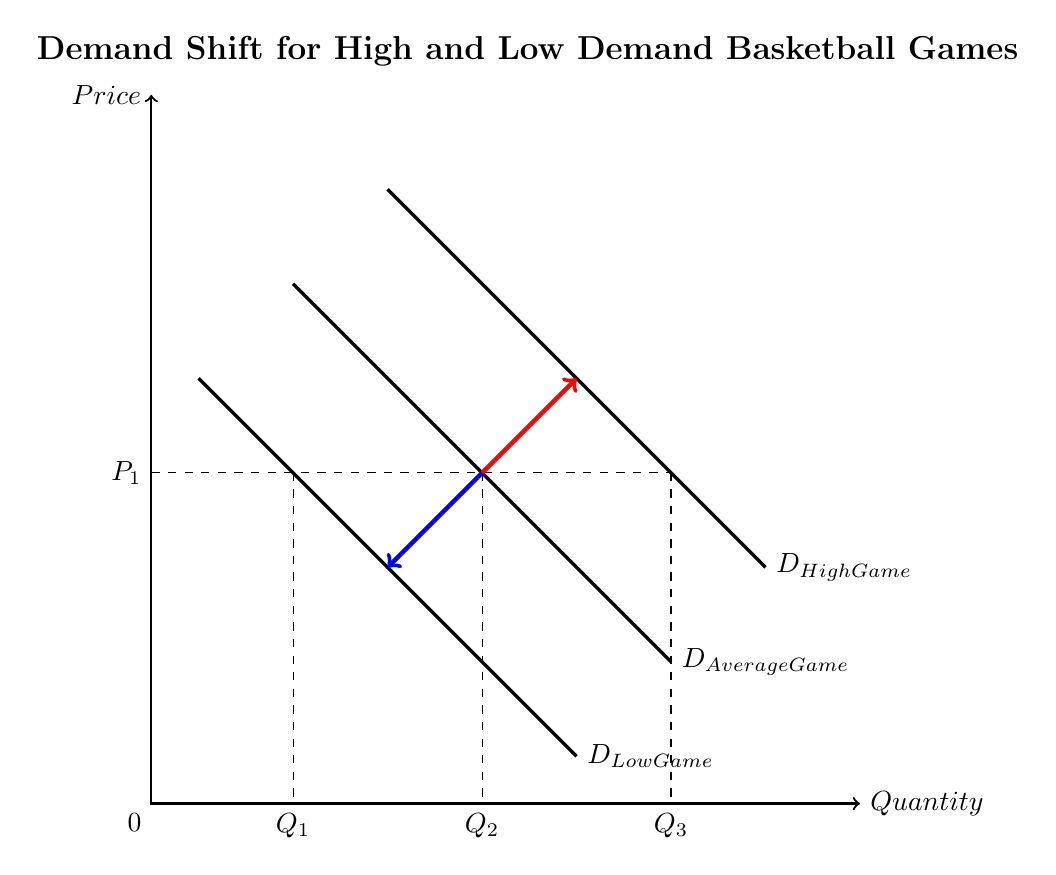
\begin{tikzpicture}[scale=0.6]
\draw[thick,<->] (0,15) node[left]{$Price$}--(0,0)--(15,0) node[right]{$Quantity$};
\node [below left] at (0,0) {$0$};
\draw[very thick](1,9)--(9,1) node[right]{$D_{Low Game}$};
\draw[very thick](3,11)--(11,3) node[right]{$D_{Average Game}$};
\node [left] at (0,7) {$P_1$};
\draw[dashed](0,7)--(11,7);
\draw[dashed](3,7)--(3,0);
\node [below] at (3,0) {$Q_1$};
\draw[dashed](7,7)--(7,0);
\node [below] at (7,0) {$Q_2$};
\draw[dashed](11,7)--(11,0);
\node [below] at (11,0) {$Q_3$};
\draw[very thick](5,13)--(13,5) node[right]{$D_{High Game}$};
\draw[->, ultra thick, red] (7,7) -- (9,9);
\draw[->, ultra thick, blue] (7,7) -- (5,5);
\node[above,font=\large\bfseries] at (current bounding box.north) {Demand Shift for High and Low Demand Basketball Games};
\end{tikzpicture}
\end{flushleft}

The blue arrow in Figure 1 shows an inward demand shift from an average basketball game to the demand for a low demand basketball game.  Likewise, the red arrow shows an outward demand shift from an average basketball game for a high demand basketball game.  In this example, all three game scenarios have the same demand slope.  Holding prices and demand determinants other than game quality constant, quantity demanded for game tickets increases from the low demand game to the average demand game to the high demand game.  $P_1$ shows a constant ticket price and $Q_1$, $Q_2$, and $Q_3$ represent the quantity demanded of tickets at price $P_1$ for each demand curve.

Figure 1 illustrates parallel demand shifts from an average game.  However, parallel demand shifts are not the only way that a demand curve can shift.  Figure 2 shows how the elasticity of demand can change at a point with a change in the slope of the demand curve.  Elasticity of demand is displayed with the slope changes.  A range of potential elasticity of demand values are shown and values range from 0 to $-\infty$.\\

\begin{large}
\ul{\textbf{Figure 2}}
\end{large}
\begin{flushleft}
\begin{large}
{\textbf{Demand Slope Change and Elasticity of Demand}}
\end{large}
\end{flushleft}\\

\includegraphics [width=12cm, height=10cm]{Picture19.png}
\begin{flushleft}
\begin{footnotesize}
{Source: https://www.e-education.psu.edu/ebf200/node/118}
\end{footnotesize}
\end{flushleft}

Figure 2 shows examples of a demand slope change without a demand shift.  Generally, the demand curve for high demand basketball games will be less responsive to price changes than the demand curve for the average basketball game.  This is displayed graphically with high demand game demand curves having a steeper slope than the average basketball game demand curve.  Likewise, the demand for lower demand basketball games is likely more responsive to price changes than the demand curve for the average basketball game.  This is displayed graphically with low demand basketball game demand curves having a flatter slope than the average basketball game demand curve.  However, all linear demand curves have areas of elastic demand, inelastic demand, and unitary elastic demand.  In Figure 2, the reported elasticity of demand for each demand curve is the intersection point for all demand curves.  Demand slope and the elasticity of demand are different concepts.  This concept is more fully discussed later.\\

\begin{large}
\ul{\textbf{Figure 3}}
\end{large}

\begin{flushleft}
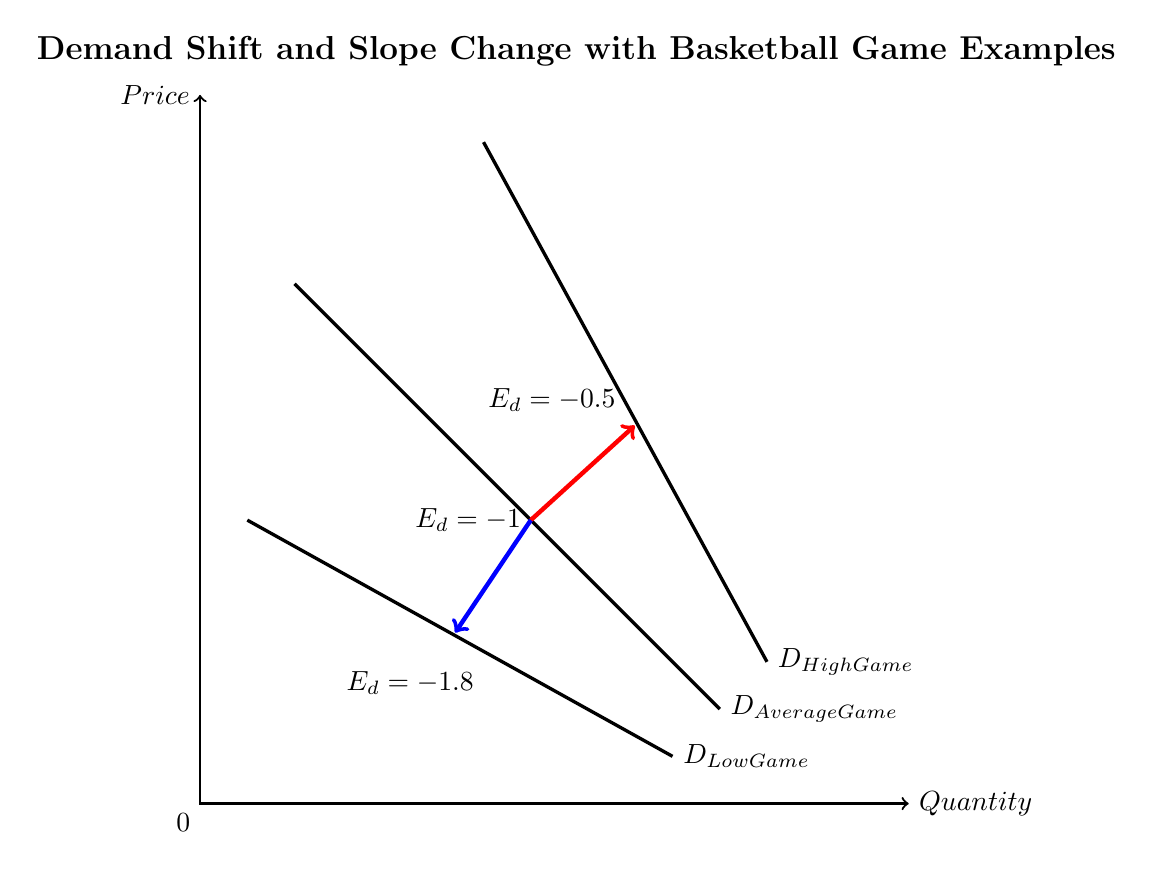
\begin{tikzpicture}[scale=0.6]
\draw[thick,<->] (0,15) node[left]{$Price$}--(0,0)--(15,0) node[right]{$Quantity$};
\node [below left] at (0,0) {$0$};
\draw[very thick](1,6)--(10,1) node[right]{$D_{Low Game}$};
\node [below left] at (6,3) {$E_d=-1.8$};
\draw[very thick](2,11)--(11,2) node[right]{$D_{Average Game}$};
\node [left] at (7,6) {$E_d=-1$};
\draw[very thick](6,14)--(12,3) node[right]{$D_{High Game}$};
\node [below left] at (9,9) {$E_d=-0.5$};
\draw[->, ultra thick, red] (7,6) -- (9.2,8);
\draw[->, ultra thick, blue] (7,6) -- (5.4,3.62);
\node[above,font=\large\bfseries] at (current bounding box.north) {Demand Shift and Slope Change with Basketball Game Examples};
\end{tikzpicture}
\end{flushleft}

Figure 3 shows a combination of a demand curve shift and a slope change of the demand curve for low and high demand basketball games relative to an average game.  This is a more realistic illustration of what happens when comparing the three game scenarios.  The low demand game has an inward shift of the demand curve and is relatively more elastic than the average season basketball game.  The high demand game has an outward shift of the demand curve and is relatively more inelastic than the average season basketball game.

\section{\textbf{Measuring Elasticity of Demand Along a Demand Curve}}

Figure 4 demonstrates that a linear demand curve has varying levels of elasticity of demand for different points on the same demand curve, despite the constant slope.  All elasticity of demand values in figure 4 are measured for the same change in quantity and the same change in price.  Figure 5 expands on the game scenarios introduced in Figure 3.  Figure 5 shows the relative location of unit elastic points for each basketball game demand curve.\\

\newpage

\begin{large}
\ul{\textbf{Figure 4}}
\end{large}

\begin{flushleft}
\begin{large}
{\textbf{Elasticity Along a Demand Curve}
\end{large}

\begin{center}
\includegraphics[width=12cm, height=7cm]{Picture72.png}
\end{center}
\begin{footnotesize}
{Source: http://www.amosweb.com/cgi-bin/awb$_$nav.pl?s=wpd&c=dsp&k=elasticity+and+demand+slope}
\end{footnotesize}
\end{flushleft}

\begin{large}
\ul{\textbf{Figure 5}}
\end{large}

\begin{flushleft}
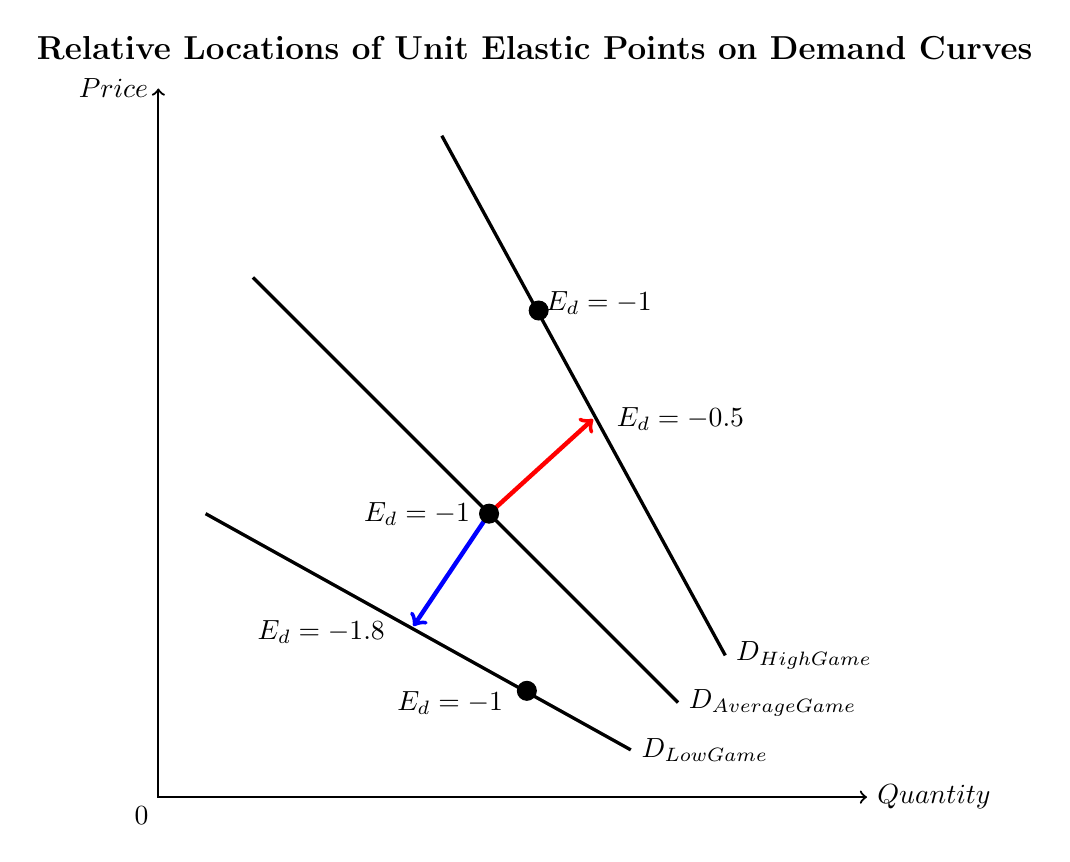
\begin{tikzpicture}[scale=0.6]
\draw[thick,<->] (0,15) node[left]{$Price$}--(0,0)--(15,0) node[right]{$Quantity$};
\node [below left] at (0,0) {$0$};
\draw[very thick](1,6)--(10,1) node[right]{$D_{Low Game}$};
\node [left] at (5,3.5) {$E_d=-1.8$};
\draw[very thick](2,11)--(11,2) node[right]{$D_{Average Game}$};
\node [left] at (6.8,6) {$E_d=-1$};
\draw[very thick](6,14)--(12,3) node[right]{$D_{High Game}$};
\node [right] at (9.5,8) {$E_d=-0.5$};
\node [left] at (7.5,2) {$E_d=-1$};
\node [above right] at (8,10) {$E_d=-1$};
\draw[->, ultra thick, red] (7,6) -- (9.2,8);
\draw[->, ultra thick, blue] (7,6) -- (5.4,3.62);
\draw [fill] (7,6) circle [radius =0.2];
\draw [fill] (8.05,10.3) circle [radius =0.2];
\draw [fill] (7.8,2.25) circle [radius =0.2];
\node[above,font=\large\bfseries] at (current bounding box.north) {Relative Locations of Unit Elastic Points on Demand Curves};
\end{tikzpicture}
\end{flushleft}

\newpage
\section{\textbf{Maximizing Revenue with Elasticity of Demand}}

\begin{large}
\ul{\textbf{Figure 6}}
\end{large}

\begin{flushleft}
\begin{large}
{\textbf{Maximizing Revenue with Elasticity of Demand}}
\end{large}
\includegraphics[width=15cm, height=10cm]{ProfitMaximization.jpg}
\end{flushleft}

\begin{footnotesize}
Source: https://courses.byui.edu/econ$_$150/econ$_$150$_$old$_$site/Lesson$_$04.htm#Section$_$01$_$Link$_$0\
\end{footnotesize}

Figure 6 illustrates a single linear demand curve with varying levels of elasticity of demand along the demand curve.  For a downward sloping linear demand curve, elasticity of demand is more elastic for higher prices along the demand curve and more inelastic for lower prices along the demand curve.  P represents price and TR represents total revenue in Figure 6. 

The point elasticity of demand of the midpoint of this demand curve is unit elastic with an elasticity of 1.  Figure 6 illustrates the fact that for a linear demand curve total revenue is maximized where the elasticity of demand has a value of 1.  If there is a shift or slope change of a demand curve, the measurements for point elasticities along the demand curve will change.  If levels of elasticity of demand change, prices must be adjusted to keep revenue at a maximized level for the new demand function.

\section{\textbf{Proposed Model of Clemson and Third Party Ticket Pricing}}

The following reasons could explain the difference in ticket prices between Clemson and third party ticket vendors for high demand basketball games. The first reason reflects differences in the organizational objectives of each institution.  Ticket vendors are profit maximizing businesses while universities are designed to enrich student experience, maintain alumni connections, and support education.  Assuming such differences in organizational objectives, third party ticket vendors and Clemson would have estimated a similar demand curve for the high demand basketball game, but Clemson would have been less willing to decrease the quantity of basketball tickets sold.  In this case, Clemson prices tickets in an effort to fill the basketball stadium rather than maximize ticket revenue.

The second reason for the difference in ticket prices is that third party ticket vendors have a better understanding of the ticket value for high demand basketball games than Clemson.  Thus Clemson under prices high demand games.  Figure 7 illustrates a situation where Clemson underestimates the demand for a high demand basketball game.  By assumption, Clemson's estimated demand curve is drawn with a flatter slope than the estimated third party demand curve.  Ticket service fees lead to more expensive third party ticket prices at all quantity levels, and there is a further difference in price caused by a difference in estimated demand slopes for the high demand basketball game.  In this example Clemson overestimates customer responsiveness to changes in ticket price.

\newpage
\begin{large}
\ul{\textbf{Figure 7}}
\end{large}

\begin{flushleft}
\begin{large}
\textbf{Model for Difference in High Demand Basketball Game Ticket Pricing}
\end{large}
\end{flushleft}

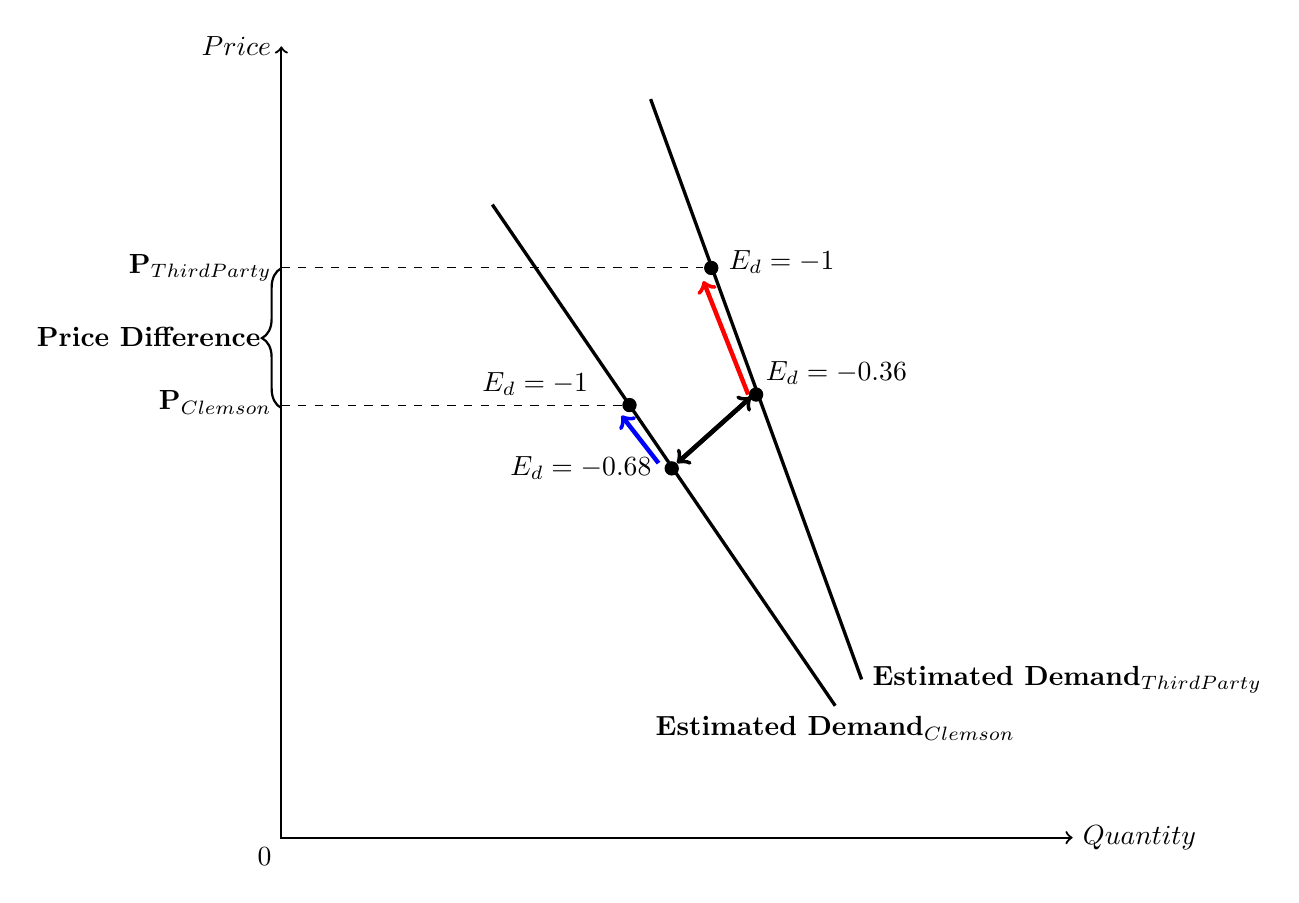
\begin{tikzpicture}[scale=0.67]
\draw[thick,<->] (0,15) node[left]{$Price$}--(0,0)--(15,0) node[right]{$Quantity$};
\node [below left] at (0,0) {$0$};
\draw[very thick](4,12)--(10.5,2.5) node[below]{\textbf{Estimated Demand$_{Clemson}$}};
\node [left] at (7.2,7) {$E_d=-0.68$};
\draw[very thick](7,14)--(11,3) node[right]{\textbf{Estimated Demand$_{Third Party}$}};
\node [right] at (9,8.8) {$E_d=-0.36$};
\draw[dashed](0,8.2)--(6.5,8.2);
\node[left] at(0,8.25){\textbf{P}$_{Clemson}$};
\draw[dashed](0,10.8)--(8,10.8);
\node[left] at (0,10.8) {\textbf{P}$_{Third Party}$};
\node [above right] at (8.3,10.5) {$E_d=-1$};
\node [above left] at (6,8.2) {$E_d=-1$};
\draw[->, ultra thick, black] (7.56,7.15) -- (8.9,8.35);
\draw[->, ultra thick, black] (8.9,8.35) -- (7.5,7.1);
\draw[->, ultra thick, red] (8.85,8.4) -- (8,10.55);
\draw [fill] (8.15,10.8) circle [radius =0.125];
\draw [fill] (6.6,8.2) circle [radius =0.125];
\draw [fill] (7.4,7) circle [radius =0.125];
\draw [fill] (9,8.4) circle [radius =0.125];
\draw[->, ultra thick, blue] (7.15,7.1) -- (6.45, 8);
\draw [decorate,decoration={brace,amplitude=7pt, mirror},xshift=0pt,yshift=-3pt, thick]
(0,10.9) -- (0,8.25) node [black, left] at (-0.2,9.6) {\textbf{Price Difference}};
\end{tikzpicture}

As shown in Figure 7, the midpoint point elasticity of Clemson's estimated demand is -0.68.  The midpoint point elasticity of demand for the third party ticket vendor is much more inelastic and has a value of -0.36.  The location and difference between the two points is shown by the double black arrow.  Clemson can maximize revenue on its estimated demand curve by pricing tickets at the unit inelastic point, shown by the blue arrow.  Third party ticket vendors can maximize revenue on its estimated demand curve by pricing tickets at the unit inelastic point, shown by the red arrow.  This would result in a ticket price difference and a total revenue difference for the high demand Clemson Basketball game.  The difference in ticket prices is displayed by the distance between P$_{ThirdParty}$ and P$_{Clemson}$.

Research with full quantity and pricing data is needed to further investigate the difference in ticket pricing strategies between Clemson and third party ticket vendors.  With that being said, a large dataset with division 1 basketball attendance information is explored in the next section of the paper to estimate the effects of several variables on Clemson Basketball game attendance.\\

\begin{Large}
\noindent\textbf{\ul{Estimating Attendance for Clemson Men's Basketball Games}}
\end{Large}
\begin{large}
\begin{enumerate}
  \item Model Selection
  \item Empirical Framework for Categorical OLS Regression
  \item Acquiring Data for Regression Model
  \item Regression Output
  \item Analysis of Regression Output
\end{enumerate}
\end{large}

\begin{large}
\setcounter{section}{0}\section{\textbf{Model Selection}}
\end{large}
\noindent
\textbf{Choosing Model}

A categorical Ordinary Least Squares (OLS) Model is selected to estimate attendance for Clemson Men's Basketball games.  An advantage of the categorical OLS model is the ease of interpretation of coefficient estimates.  A disadvantage of the categorical OLS model is that it may not fully capture trends in data.  A categorical OLS model is less robust than a traditional OLS regression model as it can only estimate a fixed number of predictions based on the zero-one values of categorical variables, whereas a traditional OLS models can provide a continuous range of predictions.  The data and data trends in Figure 8 are shown for illustration, and it should be noted that many explanatory variables do not have a strong linear relationship with the dependant variable.  OLS Models can be susceptible to underfitting a non-linear trend, or describing the trend too simply.  This is demonstrated in the high bias example of Figure 8.  Overfitting a non-linear trend is demonstrated by a more complex OLS Model in the high variance example of Figure 8.  Categorical OLS Models are less susceptible to overfitting a non-linear trend.  

The categorical OLS Model used in this paper is a low complexity model, but it is possible for the model to overfit data if the model has perfect multicollinearity.  Perfect multicollinearity occurs when all the categorical variables can be expressed as a linear combination of each other.  Thus, one category for each set of categorical variables must be omitted to avoid a singular design matrix and allow model estimation.  This means that the intercept term of the regression model is the comprehensive reference for all omitted categories of the explanatory categorical variables.\\

\begin{flushleft}
\begin{large}
\ul{\textbf{Figure 8}}
\end{large}
\includegraphics[width=17cm,height=10cm]{Picture20.png}
\begin{footnotesize}
Source: https://python-data-science.readthedocs.io/en/latest/general.html}
\end{footnotesize}
\end{flushleft}

\noindent
\textbf{Criteria for a Reasonable Regression Fit}

Bala Deshpande (2011) describes six considerations that help to ensure the statistical validity of regression models. His six points are now summarized.
\begin{enumerate}
  \item Deshpande states that most $R^2$ values in social and behavioral science models lie between 0.2 and 0.8.  He also notes that models with a $R^2$ value of less than 0.2 often lack predictive power even if individual coefficients are significant.  Moreover, models with $R^2$ values greater than 0.8 and very significant paramaters may be overfit and have poor predictive ability on new datasets.
  \item T-statistics for most included variables should be statistically significant.
  \item Error terms in the model should be normally distributed.  Most standard statistical packages do this automatically, but it is important to check that the error terms are normally distributed to assure the statistical validity of parameter t-tests.
  \item  The predictive range of a model is best near the range of the sample data used.
  \item Correlation between the independent variables and dependent variable does not imply causation.
  \item For linear regression the relationship between the independent variables and the dependent variable should be linear with respect to the estimated model parameters.
\end{enumerate}

Statistical significance is a good indicator for determining if a variable is relevant, however it should not be the only factor considered when deciding to drop a variable from the regression model.  For example, an independent categorical variable may have statistically significant coefficients if divided into five bins, but might not have statistically significant coefficients if divided into twenty bins. As the bin number increases, the bins lose differentiation, but the estimates still contain valuable information.  Another approach to checking regression validity is through the use of a QQ-plot.  A QQ-plot can be used to compare the residuals of a regression to a normal distribution.  A normal distribution of residuals suggests a constant, homoskedastic distribution of error, and is evidence of a good model fit.
    
A full explanation of the statistical properties of OLS estimators by M.G. Abbott is included in the references.  The categorical OLS Model in this paper uses an intercept term and seven independent variables that are uncorrelated with each other, but are believed to be correlated with the dependent variable.  All independent variables are integer 0-1 categorical variables.  Except for each omitted category, each team, day, month, conference affiliation, home winning percentage interval, away winning percentage interval, and betting line interval is coded as a zero/one value.  The regression estimates parameter values for all non-omitted categorical variables. Each omitted independent variable category is embedded in the regression intercept term, the baseline outcome when all other categorical variables are omitted from  the regression.

\begin{large}
\section{\textbf{Empirical Framework of Categorical OLS Regression Model}}
\end{large}

The estimated $\hat{\beta}_i$ parameter for each independent variable is the difference between the mean of the observed category and the mean of the assigned base category for the respective independent variable.  The sum of the estimated means for all omitted base categories is captured by the value of the regression constant.  This is the $\hat{\beta_0}$ estimate in the OLS model.  Any changes in game criteria, which are represented by $\hat{\beta}_i$ mean values, estimate how the dependent variable is affected by changes in independent variable categories relative to the reference category.  $Game_i$ represents the game of interest in the regression model.

\subsection{
\textbf{Empirical Ordinary Least Squares Regression Model}
}

\noindent Definition of variables:

$\bar{Y}$ = Mean value of dependent variable

$Y_i$ = Observed value of dependent variable

$\bar{X}$ = Mean value of independent variable

$X_i$ = Observed value of independent variable

$\epsilon_i$ = Error term

\noindent General OLS regression with two independent variables:
\begin{large}
\begin{equation}
Y_i = \beta_0 + \beta_1 X_i + \epsilon_i
\end{equation}
\end{large}
Sample regression line:
\begin{large}
\begin{equation}
\hat{Y}_i = \hat{\beta}_0 + \hat{\beta}_1 X_i
\end{equation}
\end{large}
Sample slope:
\begin{large}
\begin{equation}
\hat{\beta}_1 = \frac{\sum(X_i – \bar{X}) (Y_i - \bar{Y})}{\sum(X_i - \bar{X})^2}
\end{equation}
\end{large}
Sample intercept:
\begin{large}
\begin{equation}
\hat{\beta}_0 = \bar{Y}–\hat{\beta}_1 \bar{X}
\end{equation}
\end{large}
\subsection{
\textbf{Categorical Responses applied to Empirical OLS model}}

Operates like the OLS Model except variables are defined as:

$\bar{Y}$ = Mean value of dependant variable

$Y_i$ = Observed value of dependent variable

$\bar{X}$ = Mean base value of the categorical independent variable

$X_i$ = Mean value of the observed categorical independent variable

$\epsilon_i$ = Error term
\subsection{
\textbf{RSS and Model Prediction}}
\begin{large}
\begin{equation}
RSS = \sum_{i=1}^{n}(y_i-(\hat{\beta}_0 + \hat{\beta}_1 X_i))^2 = \sum_{i=1}^{n}(y_i-(\hat{y_i}))^2
\end{equation}
\end{large}

OLS estimates parameter coefficients by fitting a line through observed data points to minimize the Residual Sum of Squares (RSS).  Minimizing the RSS mathematically calculates the best possible linear data fit.  If all of the assumptions of the model are met, the parameter coefficient estimates from the regression output can be used as the basis of prediction.

\begin{large}
\section{\textbf{Acquiring Data for Regression Model}}
\end{large}

An initial dataset was collected from SportsDatabase.com.  This database is maintained by a group of researchers, data miners, and sports analysts.  A list of site maintainers and SDQL Masters can be found at: http://www.sdql.com/masters.html.

The query line used to extract the dataset used in this analysis is:
t:team, t:conference, t:school name, t:attendance, t:game number, t:season, t:month, t:line, t:wins, t:losses, o:school name,  o:wins, o:losses, o:conference, t:day, t:start time.

For the above query line approximately 65,000 college basketball games were drawn over the period 2006-2017.  The goal in extracting this information is to estimate Clemson Basketball game day attendance and identify significant explanatory factors.  A subset of the extracted data set was created, and the basketball programs of the subset schools are believed to have similar demand characteristics to Clemson Basketball.  An added benefit of selecting the sample subset was the ability to screen the data for errors.  This sampling approach was somewhat subjective.  Schools were selected based on similarity of their basketball program to Clemson, completeness of data, reported attendance within the capacity of the home school stadium, and accurate home attendance reporting.  The sample was collected with the goal of keeping the mean Clemson attendance and mean Clemson stadium capacity levels near the mean attendance and mean stadium capacity levels of the sample subset.

Clemson had a mean attendance of 7,708 and a mean stadium capacity filled level of 0.76.  The sample subset has a mean attendance of 10,255 and a mean stadium capacity filled level of 0.69.  Clemson’s mean attendance is about 25\% below the sample home attendance mean and Clemson's mean stadium capacity filled level is about 10\% above the sample stadium capacity filled mean.  It is difficult to improve the sample selection as Clemson has relatively low attendance compared to similar schools, but a relatively high percentage of stadium capacity filled.\\

\noindent
\begin{large}
\textbf{Description of Figures 9, 10, 11, and 12}
\end{large}

Figure 9 shows the number of games by conference in the sample.  Figure 10 shows the number of games by school in the sample.  Figure 11 shows the average home stadium attendance by school in the sample.  Figure 12 shows the average percent of home stadium capacity filled by school in the sample.

\newpage
\noindent
\begin{large}
\ul{\textbf{Figure 9}}
\end{large}

\noindent
\textbf{Game Observations in Sample by Conference}}\\
\includegraphics [width=\linewidth, height=5.1cm]{Image101.png}
\begin{large}
\ul{\textbf{Figure 10}}
\end{large}

\noindent
\textbf{Game Observations in Sample by School}\\
\noindent
\includegraphics [width=\linewidth, height=14.55cm]{Image99.png}

\begin{large}
\ul{\textbf{Figure 11}}
\end{large}

\noindent
\textbf{Average Attendance in Sample by School}}\\
\includegraphics [width=\linewidth, height=21cm]{Image201.png}
\newpage
\begin{large}
\ul{\textbf{Figure 12}}
\end{large}

\noindent
\textbf{Average Percent of Home Stadium Filled in Sample by School}}\\
\includegraphics [width=\linewidth, height=21cm]{301.png}

\begin{large}
\noindent\textbf{Summary of Sample Data}
\end{large}

The variable Stadium Capacity Filled was created by dividing attendance numbers by the maximum stadium capacity for each school’s home stadium.  Schools that played games at multiple home stadiums were not included in the sample.  The schools included in the sample were further screened and games with attendance reports of more than 5\% above the maximum home team stadium capacity were removed from the sample.    I reassigned reported Stadium Capacity Filled values from 1-1.05 to a value of 1 to indicate full stadium capacity for that game.

Figure 13 provides the complete summary of the sample data.  Most categorical variables can be described by their name such as Month, Day, Season, and Home School.  However, a few variables require a more complete description.  Unless "Opponent" or "Away" is included in the variable name, all variables are in relation to the home team.  The variable Home Win Percentage was created by dividing the variable Home Wins, the number of season wins of the home team at the time of $game_i$, by the variable Game Number.  The variable Game Number is defined in the SDQL database and the sample data as one more than the total games played by the home team at the time of $game_i$.  The variable Away Win Percentage was created by dividing the variable Opponent Wins, the number of season wins of the away team at the time of $game_i$, by the variable Game Number.  There are some cases where the home team and the away team played a different number of games at the time of their matchup, which would affect the respective calculations of Home Win and Away Win Percentages.  The variable ACC.Opponent designates that the home team faced an ACC opponent.  The percent of valid data for each  variable in the sample data set is reported under the column heading valid, in Figure 13.\\
\newpage
\begin{large}
\ul{\textbf{Figure 13}}
\end{large}\\

\includegraphics [width=\linewidth, height=21cm]{Picture7.png}
\newpage
\includegraphics [width=\linewidth, height=21cm]{Picture8.png}
\newpage
\includegraphics [width=\linewidth, height=21cm]{Picture9.png}
\newpage
\noindent

\begin{large}
\section{\textbf{Regression Output}}
\end{large}

\noindent
\begin{large}
\textbf{Description of Regression Output in Table 1}
\end{large}

The regression parameters reported in Table 1 are used to estimate expected attendance levels and expected stadium capacity filled levels for Clemson Men's Basketball games under specific game conditions.  The first column of Table 1 reports the parameter values for the attendance regression and the second column contains estimates for the percent of stadium capacity filled regression.  The parameter standard error is in parenthesis to the right of each parameter estimate and parameter significance level is denoted with stars.  Only the dependent variable, attendance versus percentage of stadium capacity, differs between the two estimated models.  The attendance model has an adjusted $R^2$ value of 0.247, while the stadium capacity model has an adjusted $R^2 $value of 0.3768.  The stadium capacity model also has a higher F-statistic than the attendance model.  It should be noted that if additional relevant variables were added to the model, the adjusted $R^2$ values for the attendance and stadium capacity model would likely increase.  The coefficient estimates would also likely change if more relevant variables were introduced to the model.  The reported models are intended to identify significant variables that influence Clemson Men's Basketball attendance.

The Stadium Capacity filled model is a linear model that does not bound its predictions between 0 and 1.  For very low estimates or very high estimates the Stadium Capacity Filled Model is capable of producing a dependent variable estimate below 0, or above 1.  The interpretation of an estimate less than 0 is a less that empty stadium and an estimate of more than 1 is a more than full stadium.  For this reason I recommend only using the Stadium Capacity filled model for estimating games that are not expected to sell out.  If the Stadium Capacity filled model was re-estimated, a logistic regression could be used to bound the estimates of the model between 0 and 1.  An example of the Stadium Capacity filled model estimating attendance greater than maximum stadium capacity is the North Carolina game example reported in the following empirical results section.

Eight estimated parameter values must be summed to determine the attendance and percent stadium capacity estimates for any particular game.  Game attendance and percent stadium capacity estimates are calculated by adding the constant and the appropriate parameter estimates from the following variable categories: Constant Parameter + Home is Clemson + ACC Opponent + Home Win Percentage + Away Win Percentage + Month + Day + Betting Line of Game.  The constant parameter is the reference category for all omitted dummy variable categories.  The excluded dummy variable categories consist of Clemson non-home games, Opponent Schools not in ACC, Home Win Percentage between 51-60\%, Away Win Percentage between 51-60\%, Month November, Day Thursday, and Betting Line from -5 to 5.\\

\begin{large}
\ul{\textbf{Table 1}}\hfill
\end{large}
\begin{center}{\textbf{\ul{Regression Output for Attendance and Percent Stadium Capacity Filled}}}
\begin{longtable}{@{\extracolsep{5pt}}lcc}
\\[-1.8ex]\hline 
\hline \\[-1.8ex] 
 & \multicolumn{2}{c}{\textit{Dependent variable:}} \\ 
\cline{2-3} 
\\[-1.8ex] & Attendance & Percent.Attendance \\ 
\\[-1.8ex] & (1) & (2)\\ 
\hline \\[-1.8ex] 
 Home.Clemson & $-$3,999.314$^{***}$ (369.077) & 0.025$^{*}$ (0.015)\\
 \\
 Opponent.ACCBoston College & 3,449.777$^{***}$ (399.928) & 0.155$^{***}$ (0.016) \\
 Opponent.ACCClemson & 4,359.594$^{***}$ (619.681) & 0.260$^{***}$ (0.025) \\ 
 Opponent.ACCDuke & 4,525.886$^{***}$ (387.107) & 0.252$^{***}$ 0.016)\\ 
 Opponent.ACCFlorida St & 3,518.924$^{***}$ (527.660) & 0.266$^{***}$ (0.022)\\ 
 Opponent.ACCGeorgia Tech & 2,679.664$^{***}$ (371.670) & 0.150$^{***}$ (0.015)\\ 
 Opponent.ACCLouisville & 4,062.072$^{***}$ (514.672) & 0.153$^{***}$ (0.021)\\
 Opponent.ACCMaryland & 5,355.148$^{***}$ (668.681) & 0.257$^{***}$ (0.027)\\ 
 Opponent.ACCNC State & 2,723.091$^{***}$ (399.148) & 0.154$^{***}$ (0.016) \\
 \newpage
\begin{large}
\ul{\textbf{Table 1 Continued}}\hfill
\end{large}\\
\hline \\[-1.8ex]
 Opponent.ACCNorth Carolina & 3,919.679$^{***}$ (413.015) & 0.233$^{***}$ (0.017)\\ 
 Opponent.ACCNotre Dame & 3,553.832$^{***}$ (786.032) & 0.249$^{***}$ (0.032)\\ 
 Opponent.ACCPittsburgh & 3,438.026$^{***}$ (532.808) & 0.072$^{***}$ (0.022)\\ 
 Opponent.ACCU Miami & 2,857.544$^{***}$ (393.583) & 0.150$^{***}$ (0.016)\\ 
 Opponent.ACCVirginia & 2,485.684$^{***}$ (411.116) & 0.154$^{***}$ (0.017)\\ 
 Opponent.ACCWake Forest & 2,824.667$^{***}$ (406.734) & 0.146$^{***}$ (0.017)\\ 
 \\
 Home.Win.Percentage=\textless 40\% & $-$1,222.191$^{***}$ (253.621) & $-$0.053$^{***}$ (0.010)\\ 
 Home.Win.Percentage41-50\% & $-$40.511 (202.395) & 0.007 (0.008)\\
 Home.Win.Percentage\textgreater 61-70\% & 566.117$^{***}$ (175.546) & 0.038$^{***}$ (0.007)\\ 
 Home.Win.Percentage71-80\% & 1,427.477$^{***}$ (195.960) & 0.067$^{***}$ (0.008)\\ 
 Home.Win.Percentage\textgreater 80\% & 1,699.217$^{***}$ (259.900) & 0.080$^{***}$ (0.011)\\
 \\
 Away.Win.Percentage=\textless 40\% & $-$1,038.923$^{***}$ (247.086) & $-$0.046$^{***}$ (0.010)\\
 Away.Win.Percentage41-50\% & $-$369.479$^{*}$ (215.431) & $-$0.019$^{**}$ (0.009)\\ 
 Away.Win.Percentage\textgreater 61-70\% & 670.894$^{***}$ (187.755) & 0.024$^{***}$ (0.008)\\ 
 Away.Win.Percentage71-80\% & 1,208.252$^{***}$ (200.837) & 0.041$^{***}$ (0.008)\\ 
 Away.Win.Percentage\textgreater 80\% & 1,896.644$^{***}$ (254.473) & 0.075$^{***}$ (0.010)\\ 
 \\           
 MonthJanuary & 2,019.473$^{***}$ (242.051) & 0.149$^{***}$ (0.010)\\ 
 MonthFebruary & 2,690.293$^{***}$ (242.269) & 0.177$^{***}$ (0.010)\\ 
 MonthMarch & 1,976.336$^{***}$ (281.499) & 0.125$^{***}$ (0.012)\\ 
 MonthDecember & 1,052.092$^{***}$ (242.297) & 0.079$^{***}$ (0.010)\\
 \\
 DayFriday & 140.783 (388.287) & 0.021 (0.016)\\
 \begin{large}
\ul{\textbf{Table 1 Continued}}
\end{large}\\
\hline \\[-1.8ex]
 DayMonday & $-$173.781 (328.429) & $-$0.044$^{***}$ (0.013)\\ 
 DaySaturday & 1,268.855$^{***}$ (231.226) & 0.054$^{***}$ (0.009)\\ 
 DaySunday & 698.412$^{**}$ (281.007) & 0.021$^{*}$ (0.011)\\ 
 DayTuesday & 602.625$^{**}$ (256.738) & $-$0.016 (0.010)\\ 
 DayWednesday & $-$149.547 (245.776) & $-$0.023$^{**}$ (0.010)\\ 
\\
Betting.Line12-18pt.Underdog & 1,936.147$^{***}$ (213.743) & 0.047$^{***}$ (0.009)\\ 
Betting.Line5-11pt.Underdog & 783.234$^{***}$ (154.994) & 0.015$^{**}$ (0.006)\\ 
Betting.Line5-11pt.Favorite & $-$1,013.454$^{***}$ (233.794) & $-$0.025$^{**}$ (0.010)\\
Betting.Line12-18pt.Favorite & $-$1,181.368$^{***}$ (449.247) & $-$0.005 (0.018)\\
Constant & 5,967.257$^{***}$ (361.066) & 0.478$^{***}$ (0.015)\\ 
\hline \\[-1.8ex] 
Observations & 5,006 & 5,006 \\ 
R$^{2}$ & 0.281 & 0.392 \\ 
Adjusted R$^{2}$ & 0.276 & 0.387 \\ 
Residual Std. Error (df = 4966) & 4,187.450 & 0.171 \\ 
F Statistic (df = 39; 4966) & 49.814$^{***}$ & 82.148$^{***}$ \\ 
\hline 
\hline \\[-1.8ex] 
\textit{Note:}  & \multicolumn{2}{r}{$^{*}$p$<$0.1; $^{**}$p$<$0.05; $^{***}$p$<$0.01} \\ 
\end{longtable}
\end{center}

\newpage
\noindent
\begin{large}
\textbf{Description of Figures 14, 15, 16, and 17}
\end{large}

Point 3 from the regression validity article states: "Error terms in the model should be normally distributed. Most standard statistical packages do this automatically, but it is good to know that this check has been performed."  Figures 14, 15, 16, and 17 are heuristics used to examine the regression assumption of a normal distribution of residuals.  The residual distribution for both the mean attendance and mean stadium capacity models are approximately normally distributed.

Figure 15 shows that the attendance regression has a higher concentration of residuals at high attendance values compared to a normal distribution.  This may have been caused from the process used to select the data sample.  Stadium capacity estimates in the 1-1.05 range were kept as these values were determined to be within a reasonable amount of the maximum capacity of each school's home stadium.  However, attendance for games where attendance exceeded capacity by up to 5 percent were adjusted downward to 100 percent full stadium capacity when estimating the stadium capacity model.  In contrast, the corresponding attendance values in the attendance model were not adjusted.  This is a possible explanation for the high concentration of residuals for high values in the attendance regression, and the more normal distribution of residuals for high values in the stadium capacity filled regression.

\newpage
\noindent
\begin{large}
\ul{\textbf{Figure 14}}
\end{large}\\

\includegraphics [width=\linewidth, height=9cm]{Picture14.png}
\begin{large}
\ul{\textbf{Figure 15}}
\end{large}\\

\includegraphics [width=\linewidth, height=10cm]{Picture15.png}
\newpage
\noindent
\begin{large}
\ul{\textbf{Figure 16}}
\end{large}\\

\includegraphics [width=\linewidth, height=9cm]{Picture17.png}
\begin{large}
\ul{\textbf{Figure 17}}
\end{large}\\

\includegraphics [width=\linewidth, height=10cm]{Picture18.png}
\newpage

\begin{large}
\section{\textbf{Analysis of Regression Output}}
\end{large}
\subsection{\textbf{Attendance Estimates for Game Scenarios}}
Assume that an average attendance Clemson Basketball game can be estimated for a Clemson vs. NC State basketball game.  The game is on a Tuesday in January, Clemson is expected to have a 61-70 win percentage, and NC State is expected to have a 51-60 win percentage when the game is played.  Clemson is an expected 4 point favorite for the game.

Lets further assume an above average attendance Clemson basketball game can be estimated for a Clemson vs. North Carolina basketball game.  The game is on a Friday in February, North Carolina is expected to have a 71-80 win percentage, and Clemson is expected to have a 61-70 win percentage when the game is played.  Clemson is an expected 8 point underdog for the game.

Finally, lets assume a below average attendance Clemson Basketball game can be estimated for a Clemson vs. Pittsburgh basketball game.  The game is on a Wednesday in December, Clemson is expected to have a 61-70 point win percentage, and Pittsburgh is expected to have a 41-50 win percentage when the game is played.  Clemson is an expected 8 point favorite for the game.

Below are the attendance and percent stadium capacity filled estimates for the NC State game, North Carolina game, and Pittsburgh game for each scenario defined.  All of the values are taken from Table 1, which contains the regression parameter estimates for both the attendance and percent stadium capacity filled models.\\

\noindent\textbf{Clemson vs. NC State Men's Basketball Game Estimates}\\
\noindent
$\hat{Y_i}$ = Home.Clemson + Opponent.ACCNC State + Home.Win.Percentage61-70\\ + Away.Win.Percentage51-60 + MonthJanuary + DayTuesday + EvenBettingLine + Constant

\noindent$\hat{Y_a}$ = (-3999)+(2723)+(566)+(0)
+(2019)+(602)+(0)+(5967) = \textbf{7,878} Attendants

\noindent$\hat{Y_s}$ = (.025) + (.154)+(.038)+(0)+(0.149)+(-.016)+(0)+(0.478) =  \textbf{82.8\%} Stadium Capacity Filled\\

\newpage
\noindent\textbf{Clemson vs. North Carolina Men's Basketball Game Estimates}\\
\noindent
$\hat{Y_i}$ = Home.Clemson + Opponent.ACC.North Carolina + Home.Win.Percentage61-70 \\+ Away.Win.Percentage71-80 + MonthFebruary + DayFriday + BettingLine5-11pt.Underdog + Constant

\noindent$\hat{Y_a}$ = (-3999)+(3919)+(566)+(1208)
+(2690)+(140)+(784)+(5967) = \textbf{11,545} Attendants

\noindent$\hat{Y_s}$ = (.025)+(.233)+(.038)+(.041)
+(0.177)+(0.021)+(.015)+(0.478)\\  = \textbf{102.8\%}** Stadium Capacity Filled\\
**Regression estimates expected attendance to exceed maximimum stadium capacity.\\

\noindent\textbf{Clemson vs. Pittsburgh Men's Basketball Game Estimates}\\
\noindent
$\hat{Y_i}$ = Home.Clemson + Opponent.ACC.Pittsburgh + Home.Win.Percentage61-70\\ + Away.Win.Percentage41-50 + MonthDecember + DayWednesday + BettingLine5-11pt.Favorite + Constant

\noindent$\hat{Y_a}$= (-3999)+(3438)+(566)+(-369)
+(1052)+(-150)+(-1013)+(5967) = \textbf{5,492} Attendants

\noindent$\hat{Y_s}$= (.025)+(.072)+(.038)+(-0.019)
+(0.079)+(-0.023)+(-0.025)+(0.478)\\  = \textbf{62.5\%} Stadium Capacity Filled

\begin{large}
\subsection{\textbf{Discussion of Regression Model Variable Estimates}}
\end{large}

Zero values in the above estimates correspond to the omitted parameter categories.  Estimated attendance and stadium capacity filled levels for the base month November are lower than for other months.  The primary reason for this is likely because conference play doesn't start until later in the season and the games in the month of November are less competitive than games in other months.  Some of the category estimates for ACC opponents seem counterintuitive.  A possible explanation is that ACC schools that are thought to be good programs also have very competitive win records, and the variable opponent win record could be capturing some of the estimated attendance and stadium capacity values for competitive ACC opponents.  An example is that Pittsburgh has a higher ACC opponent estimate than Virginia in the attendance model.  However, Pittsburgh usually has a weak losing record and Virginia usually has a strong winning record.
\newpage
\begin{large}
\noindent\textbf{Conclusion and Areas of Further Research}
\end{large}

The regression output from Table 1 was used to estimate game day attendance and the percent of stadium capacity filled, but the model may have weak predictive ability.  Several variables are significant when estimating levels of attendance and stadium capacity filled, but the stability of the coefficient estimates needs to be tested by adding other relevant variables to each model.  If the regression framework was used to estimate demand and elasticity of demand, additional data on ticket prices would be needed.  If the ticket pricing decision maker knew average game attendance and average ticket price, and if an elasticity of demand value could be derived for Clemson home games, then the elasticity value in combination with predicted home game attendance from the estimated quantity models could be used to estimate the revenue maximizing ticket price.  In its current form the quantity regression models are not recommended for prediction, but the analysis confirms the influence of several variables on Clemson Men's Basketball home game attendance.

The only way to determine if schools like Clemson are pricing tickets intentionally below third party ticket vendors is by analyzing school datasets with pricing information.  A difference in demand estimates for a given basketball game could explain the difference in revenue maximizing ticket price levels.  My intuition is that third party ticket vendors estimate high demand basketball games to be more inelastic than the demand estimates of schools. However, pricing differences could also be attributed to differences in organizational goals.
\newpage
\noindent
\begin{Large}
\textbf{References}
\end{Large}\\

\noindent Abbott, M.G. “Note 4: Statistical Properties of the OLS Coefficient Estimators.” Economics 351* Introductory Econometrics, Queen's University, qed.econ.queensu.ca/pub/faculty/abbott/econ351/351note04.pdf.\\

\noindent Boyd, D.W. & Boyd, L.A. J Econ Finan (1996)  20: 23. https://doi.org/10.1007/BF02920889\\

\noindent Cameron, S. (2002). Bruins to set prices hourly. Sports Business Journal, pp. 1,
50.\\

\noindent Coates, Dennis \& Humphreys, Brad. (2007). Ticket Prices, Concessions and Attendance at Professional Sporting Events. International Journal of Sport Finance. 2. 161-170.\\

\noindent Demmert, Henry G. (1973). The Economics of Professional Team Sports. Lexington, Mass. D.C. Heath & Co..\\ 

\noindent Deshpande, Bala. (2011). “6 Checkpoints to Ensure Regression Model Validity for Analytics.” Analytics Made Accessible: for Small and Medium Business and Beyond,
www.simafore.com/blog/bid/54963/6-checkpoints-to-ensure-regression-model-validity-for-analytics.\\

\noindent Dilts, David. (2004). Introduction to Microeconomics. Fort Wayne, Indiana.  Indiana - Purdue University,
https://www.pfw.edu/dotAsset/142427.pdf
\\ 
 
\noindent Feehan, Patrick. (2006).  “Chapter 9 Attendance at Sports Events.” Handbook on the Economics of Sports. pp. 90–99, 
www.ahmetguvener.com/wp-content/uploads/Handbook-on-the-Economics-of-Sport.pdf#page=109.\\

\noindent Fort, Rodney. (2004). Inelastic sports pricing. Managerial and Decision Economics. 25. 87-94.\\

\noindent Jennet, N. (1984), Attendances, Uncertainty of Outcome and Policy in Scottish League Football.  Scottish Journal of Political Economy, 31: 176-198.\\

\noindent Noll, Roger G. (1974). Government and the Sports Business: Papers prepared for a conference of experts, with an introduction and summary. No. 8. Brookings institution.\\

\noindent Rascher, Daniel \& McEvoy, Chad \& Nagel, Mark \& Brown, Matthew. (2007)  “Variable ticket pricing in Major League Baseball.”Journal of Sport Management, Vol. 21. p. 407-437.\\

\noindent Scully, Gerald W. 1989. The Business of Major League Baseball. Chicago: University of Chicago Press.\\

\noindent Villar, Jaume \& Guerrero, Plácido. (2009). "Sports attendance: A survey of the Literature 1973-2007," Rivista di Diritto ed Economia dello Sport, Centro di diritto e business dello Sport, vol. 5(2), pages 111-151, Settembre,
https://core.ac.uk/download/pdf/6396808.pdf

\end{document}
